\documentclass{beamer}
\usepackage{etex}

\usepackage{soul}

% TABLES
\newcommand{\ra}[1]{\renewcommand{\arraystretch}{#1}} % spaces in tables
\usepackage{booktabs}   % Allows the use of \toprule, \midrule and \bottomrule in tables for horizontal lines

% LISTS
% \usepackage{enumitem} % Changes the itemize and enumerate


% PSTRICKS
% \usepackage{pstricks,pst-node,pst-tree} % includes graph additions
% \usepackage{pst-pdf} % Compiles the pictures
% \usepackage{pst-node}
% \usepackage{pst-plot}
% \psset{xunit=1cm,yunit=1cm}


% INCLUDE GRAPHICS
\usepackage{graphicx}


% LOGO POSITION
\usepackage{pgf}
% \usepackage[absolute,overlay]{textpos}


% FONTS
% \usefonttheme{serif}
\usefonttheme[onlymath]{serif} % Standard font for math enviroments
\usepackage[T1]{fontenc}
%\usepackage{inconsolata} % Nice monospaced font



% CODE
\usepackage{listings} % Code block (source code) \begin{lstlisting} 

\lstset{
    language=Python,                        % Code langugage
    commentstyle=\color{gray},              % Comments font
    basicstyle=\small\ttfamily,             % Code font, Examples: \footnotesize, \ttfamily
    keywordstyle=\bfseries\color{blue},
    stringstyle=\color{orange},
    numbers=left,                           % Line nums position
    numberstyle=\tiny,                      % Line-numbers fonts
    stepnumber=1,                           % Step between two line-numbers
    numbersep=5pt,                          % How far are line-numbers from code
    numbers=none,
    frame=single,                             % A frame around the code
    tabsize=4,                              % Default tab size
    captionpos=b,                           % Caption-position = bottom
    breaklines=true,                        % Automatic line breaking?
    breakatwhitespace=false,                % Automatic breaks only at whitespace?
    showspaces=false,                       % Dont make spaces visible
    showstringspaces=false,                 % Dont make spaces visible in strings
    showtabs=false,                         % Dont make tabls visible
    belowskip=8pt,
    morekeywords={range, xrange},
    backgroundcolor=\color{white}
    % emph={[2]root,base}
    % morekeywords={one,two,three,four,five,six,seven,eight,
}



\newcommand{\code}[1]{{\small\ttfamily #1}} % \code{inline code}


% BEAMER COLORS
\definecolor{kugreen}{RGB}{50,93,61}
\setbeamercolor{frametitle}{fg=black}
\setbeamercolor{normal text}{fg=black}
\setbeamercolor{structure}{fg=kugreen}

% BEAMER STYLE
\setbeamertemplate{itemize item}{$\bullet$}
\setbeamersize{text margin left=10pt}
\setbeamersize{text margin right=10pt}
\setbeamersize{sidebar width right=0pt}
\setbeamersize{sidebar width left=0pt}
\setbeamercolor{block title}{fg=white,bg=kugreen}
\setbeamercolor{block body}{fg=black,bg=white!95!black}


% BEAMER HEADLINE
\setbeamertemplate{headline}
{%
    % \vbox{

    % \vspace{2pt}

    % \hspace{10pt}
    % \tiny
    % \rmfamily
    % \expandafter\insertshortauthor
    %     \vspace{1pt}
    % }
}


% BEAMER TITLE
\setbeamertemplate{frametitle}
{
    \color{kugreen}
    \begin{centering}\medskip
        \insertframetitle\par
    \end{centering}
}


% BEAMER FOOTER
\setbeamertemplate{footline}[text line]
{%
    \vbox{%
        \tiny\ttfamily
        \insertvrule{0.5pt}{kugreen}

        \vspace{2pt}

        \strut{
        \rmfamily\itshape
        \expandafter\insertshorttitle
        \expandafter\insertauthor,
        \insertshortinstitute
        }
        \hfill\strut{
        }
        \hfill\strut{
            \insertframenumber\,/\,\inserttotalframenumber
            % 
\includegraphics[width=20pt,natwidth=610,natheight=642]{KUNATLogo.pdf}
        }

        \vspace{1pt}
    }
}

\setbeamertemplate{background}{
    % \hspace{330pt}
\includegraphics[width=25pt,natwidth=610,natheight=642]{KUNATLogo.pdf}
}

% BEAMER Frontpage
\setbeamertemplate{title page}
{

    \begin{beamercolorbox}[center]{beamer color}

        {
            \huge
            \color{kugreen}
            \inserttitle
        }
        \bigskip
        \bigskip

        
\includegraphics[width=2cm]{KUNATLogo}

        \bigskip
        {
            \bf
            \rmfamily
            {\large \insertauthor}
        }

        \smallskip
        {
            \rmfamily
            \footnotesize
            \insertinstitute
        }

        {
            \rmfamily
            \footnotesize
            \insertdate
        }

    \end{beamercolorbox}


    \addtocounter{framenumber}{-1}
}

% Removes the navigation bar
\beamertemplatenavigationsymbolsempty

% CONTENT

\logo{\pgfputat{\pgfxy(-1,-0.435)}{\pgfbox[center,base]{
\includegraphics[width=1.2cm,natwidth=610,natheight=642]{KUNATLogo.pdf}}}}




% TITLE AND OTHER STUFF GOES HERE
\title[University of Copenhagen]{Molecular Statistics, Exam Projects}
\author{
    % Jimmy C. Kromann - jimmy@charnley.dk
    % \newline
    % Lars A. Bratholm - larsbratholm@gmail.com\\
}

\date{2015}

\begin{document}

\frame[plain]{\titlepage}


% ***************************************************
% BEGIN FRAMES
% ***************************************************

\frame
{
    \frametitle{Projects}

    \begin{enumerate}
      \item Diffusion Coefficient of the Lennard-Jones Fluid {\bf (JCK)}
      \item Genetic Algorithm {\bf (JCK)}
      \item Ising Spin-Lattice {\bf (LAB)}
      \item Chemical Shifts Study {\bf (LAB)}
    \end{enumerate}
}

\frame
{
    \frametitle{Project 1: Diffusion Coefficient}
    \centering

    Self-diffusion in Lennard-Jones Fluid.
    \newline

    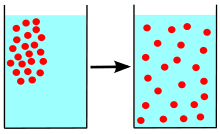
\includegraphics[width=0.2\textwidth]{images/diffusion_illustration.png}

    \begin{columns}[c]
      \column{0.5\textwidth}
      \centering

        Mean-Square Displacement

        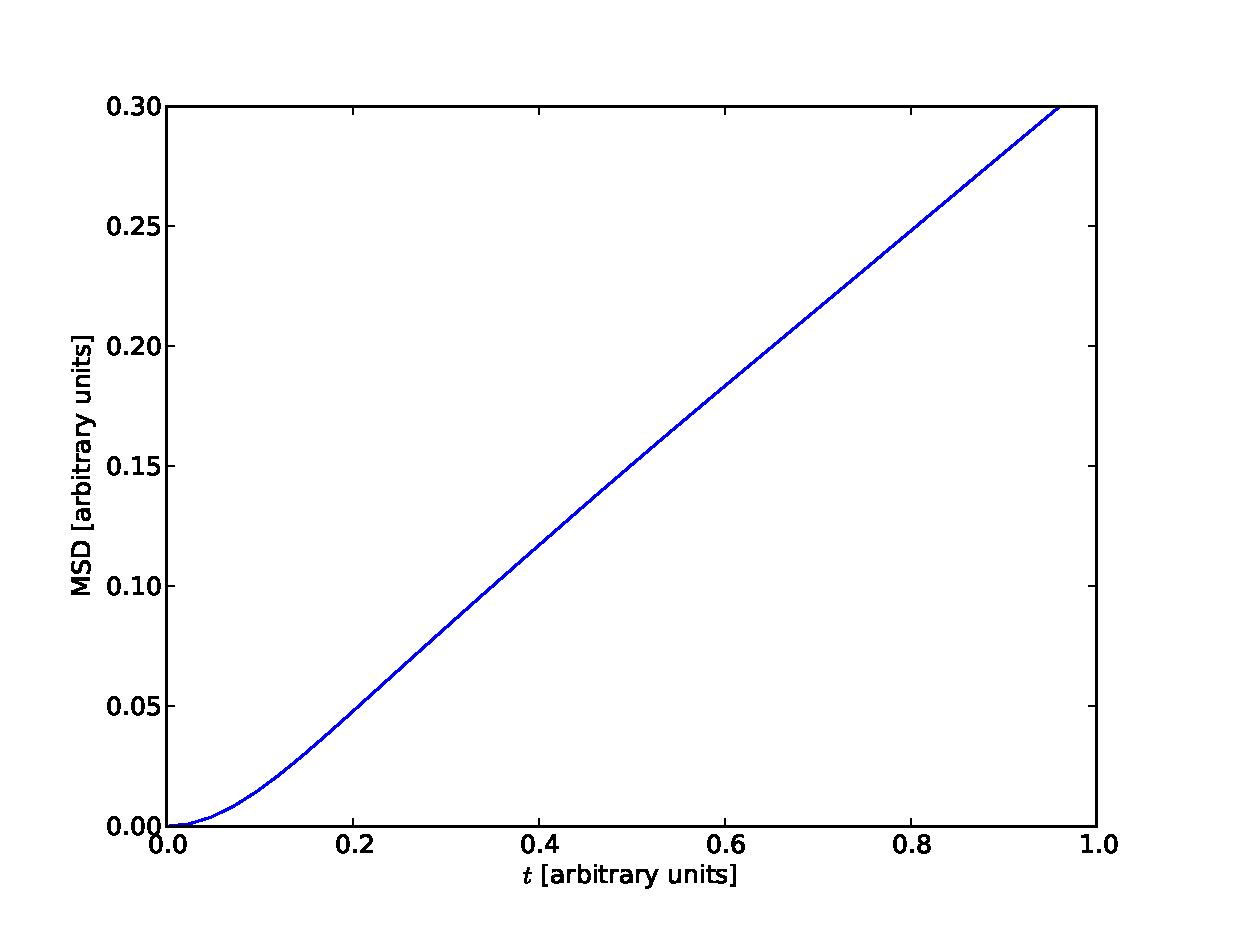
\includegraphics[width=0.8\textwidth]{images/diffusion_msd.eps}

      \column{0.5\textwidth}
      \centering

        Velocity Auto-Correlation Function

        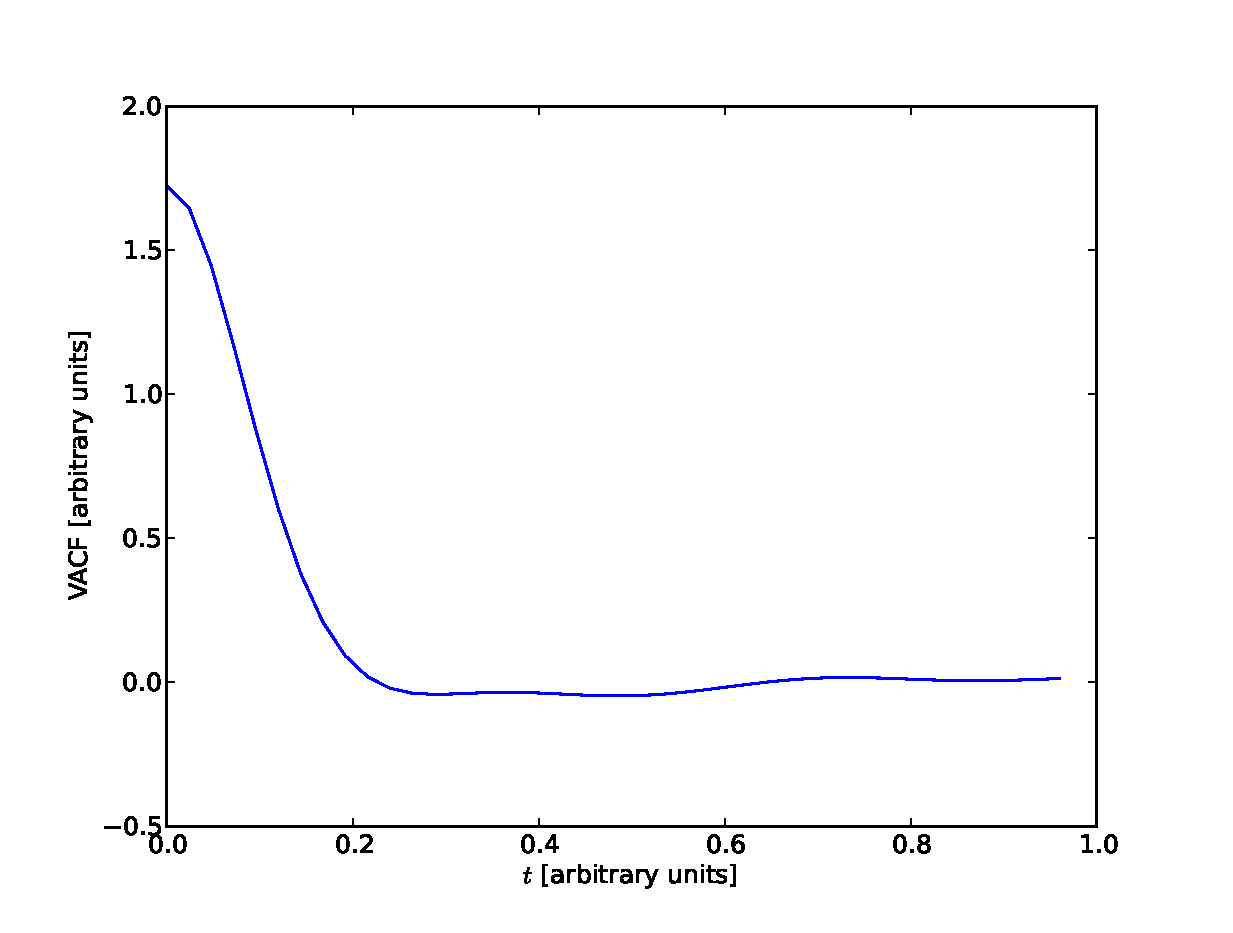
\includegraphics[width=0.8\textwidth]{images/diffusion_vacf.eps}

    \end{columns}

    \begin{align*}
        D \ \ = \ \ \lim_{t\rightarrow \infty} \frac{\mathrm{MSD}(t)}{4t}
          \ \ = \ \ \frac{1}{2} \int_0^\infty \mathrm{VACF}(t) \ \ dt
    \end{align*}

}


\frame
{
  \frametitle{Project 1: Diffusion Coefficient}
  {\bf Project description:}

  \smallskip

  \begin{itemize}
    \item Simulate diffusion under different simulation conditions
            (pressure, temperature, etc.) using MD in Python.
    \vspace{0.2in}
    \item Calculate MSD and VACF.
    \vspace{0.2in}
    \item Calculate diffusion coefficients.
  \end{itemize}

}


\frame
{
    \frametitle{Project 2: Genetic Algorithm}

    \centering
    {\bf Genetic Algorithm}

    \begin{center}
        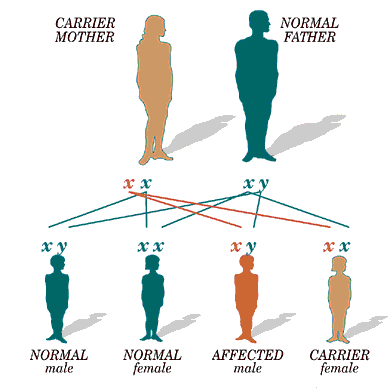
\includegraphics[width=0.5\textwidth]{images/genetics_family.png}
    \end{center}
}


\frame
{
    \frametitle{Project 2: Genetic Algorithm}

    \begin{center}
    Energy as a function of dihedral angles
    \end{center}

    \begin{columns}[c]
      \column{0.5\textwidth}

\begin{figure}
	\psset{xunit=0.8cm,yunit=0.8cm}
    \begin{pspicture}(-2,-3)(4,3)
        \psframe(-2,-3)(4,3)
        \psline{->}(0.0,0.0)(2.0,0.0)
        \rput{60.0}(0.0,0.0)
        {
            \psline{->}(-2.0,0.0)(0.0,0.0)
            \pscircle(-2.0,0.0){0.3}
        }
        \rput{60.0}(2.0,0.0)
        {
            \psline{->}(0.0,0.0)(2.0,0.0)
            \pscircle(2.0,0.0){0.3}
        }

        % Circles
        \pscircle(0.0,0.0){0.3}
        \pscircle(2.0,0.0){0.3}
        \rput(3.0,0.0){.}
        \psellipse[linestyle=dashed](3.0,0.0)(0.2,1.7)
        \psellipse[linestyle=dashed](1.0,0.0)(0.15,0.6)
        \psframe*[linecolor=white](0.84,0.1)(1.16,0.7)
        \parabola{->}(0.85,0.0)(1.0,0.6)
        \rput(1.15,0.8){$\omega$}
        \rput(-1.5, -1.4){A}
        \rput(-0.4, 0.4){B}
        \rput(2.0, -0.6){C}
        \rput(2.6, 2.1){D}
    \end{pspicture}
\end{figure}

        \column{0.5\textwidth}

            \centering

            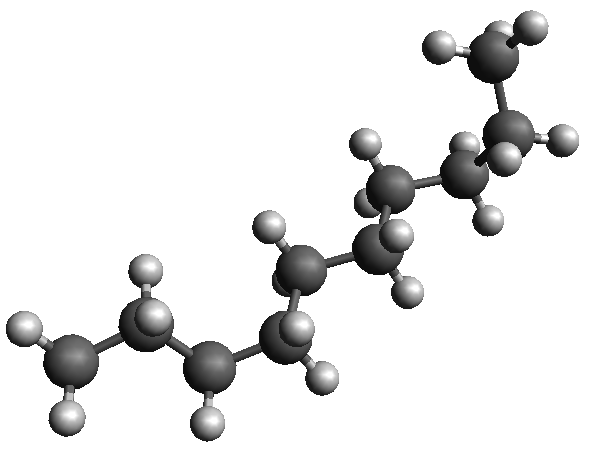
\includegraphics[width=0.8\textwidth]{images/genetics_unsorted.png}


    \end{columns}

}


\frame
{
    \frametitle{Project 2: Genetic Algorithm}

    \begin{columns}[c]
      \column{0.5\textwidth}
      \centering
      Parent

      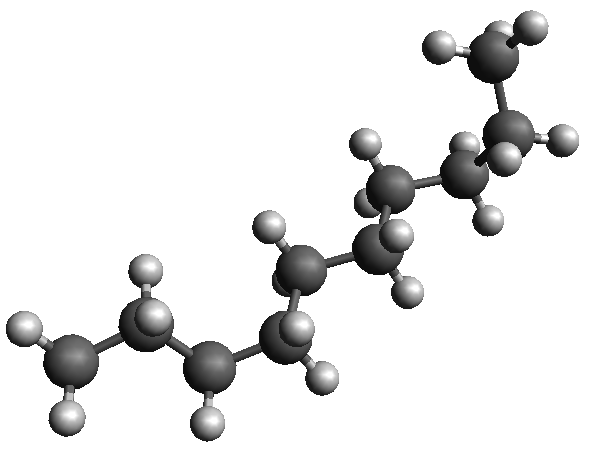
\includegraphics[width=0.4\textwidth]{images/genetics_unsorted.png}

      High energy

      \column{0.5\textwidth}
      \centering
      Child

      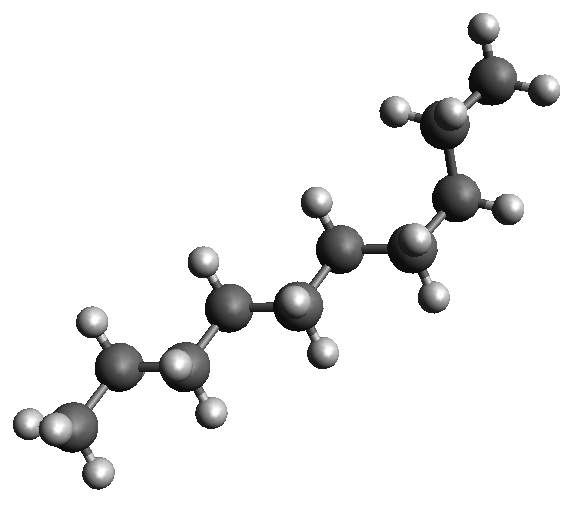
\includegraphics[width=0.4\textwidth]{images/genetics_sorted.png}

      Low energy

    \end{columns}

    \qquad
    \newline
    \qquad

    {\bf Project description:}
    \begin{itemize}

        \item Implement the genetic algorithm in Python.

        \smallskip

        \item Use a force field to calculate molecular energies.

        \smallskip

        \item Use the genetic algorithm to energy minimize alkane 
                molecular structures.

    \end{itemize}
}

\frame
{
    \frametitle{Project 3: 2D Ising Model}

    \begin{center}
        Representation of 2D magnetic solid
    \end{center}

    \bigskip

    \begin{columns}[c]

        \column{0.5\textwidth}

            \centering
        
            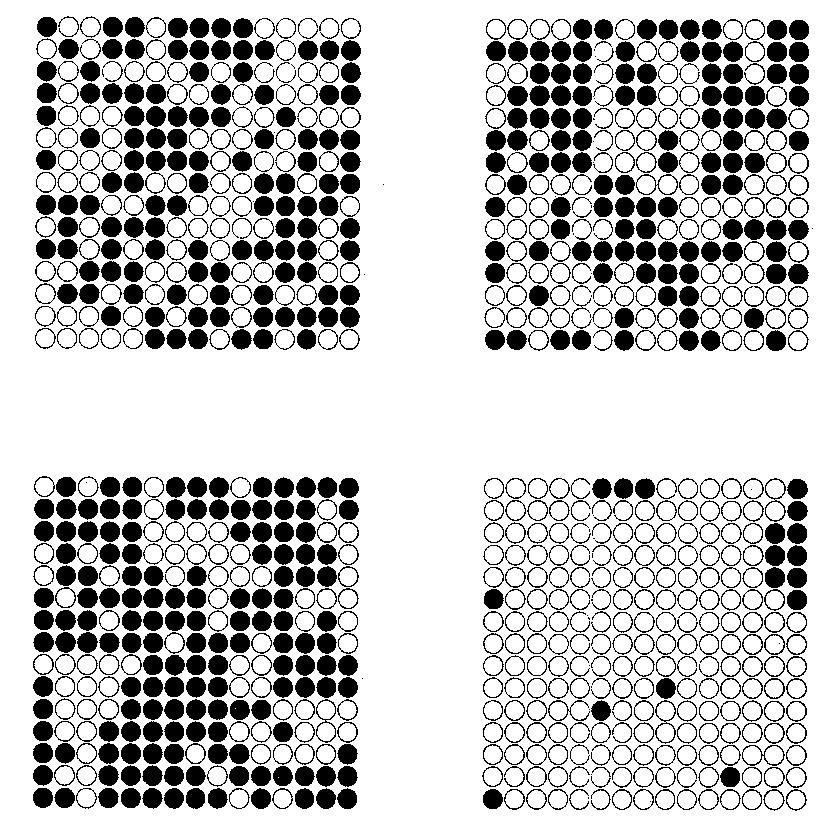
\includegraphics[width=0.9\linewidth]{temperatures.jpg}


        \column{0.5\textwidth}

            \centering

            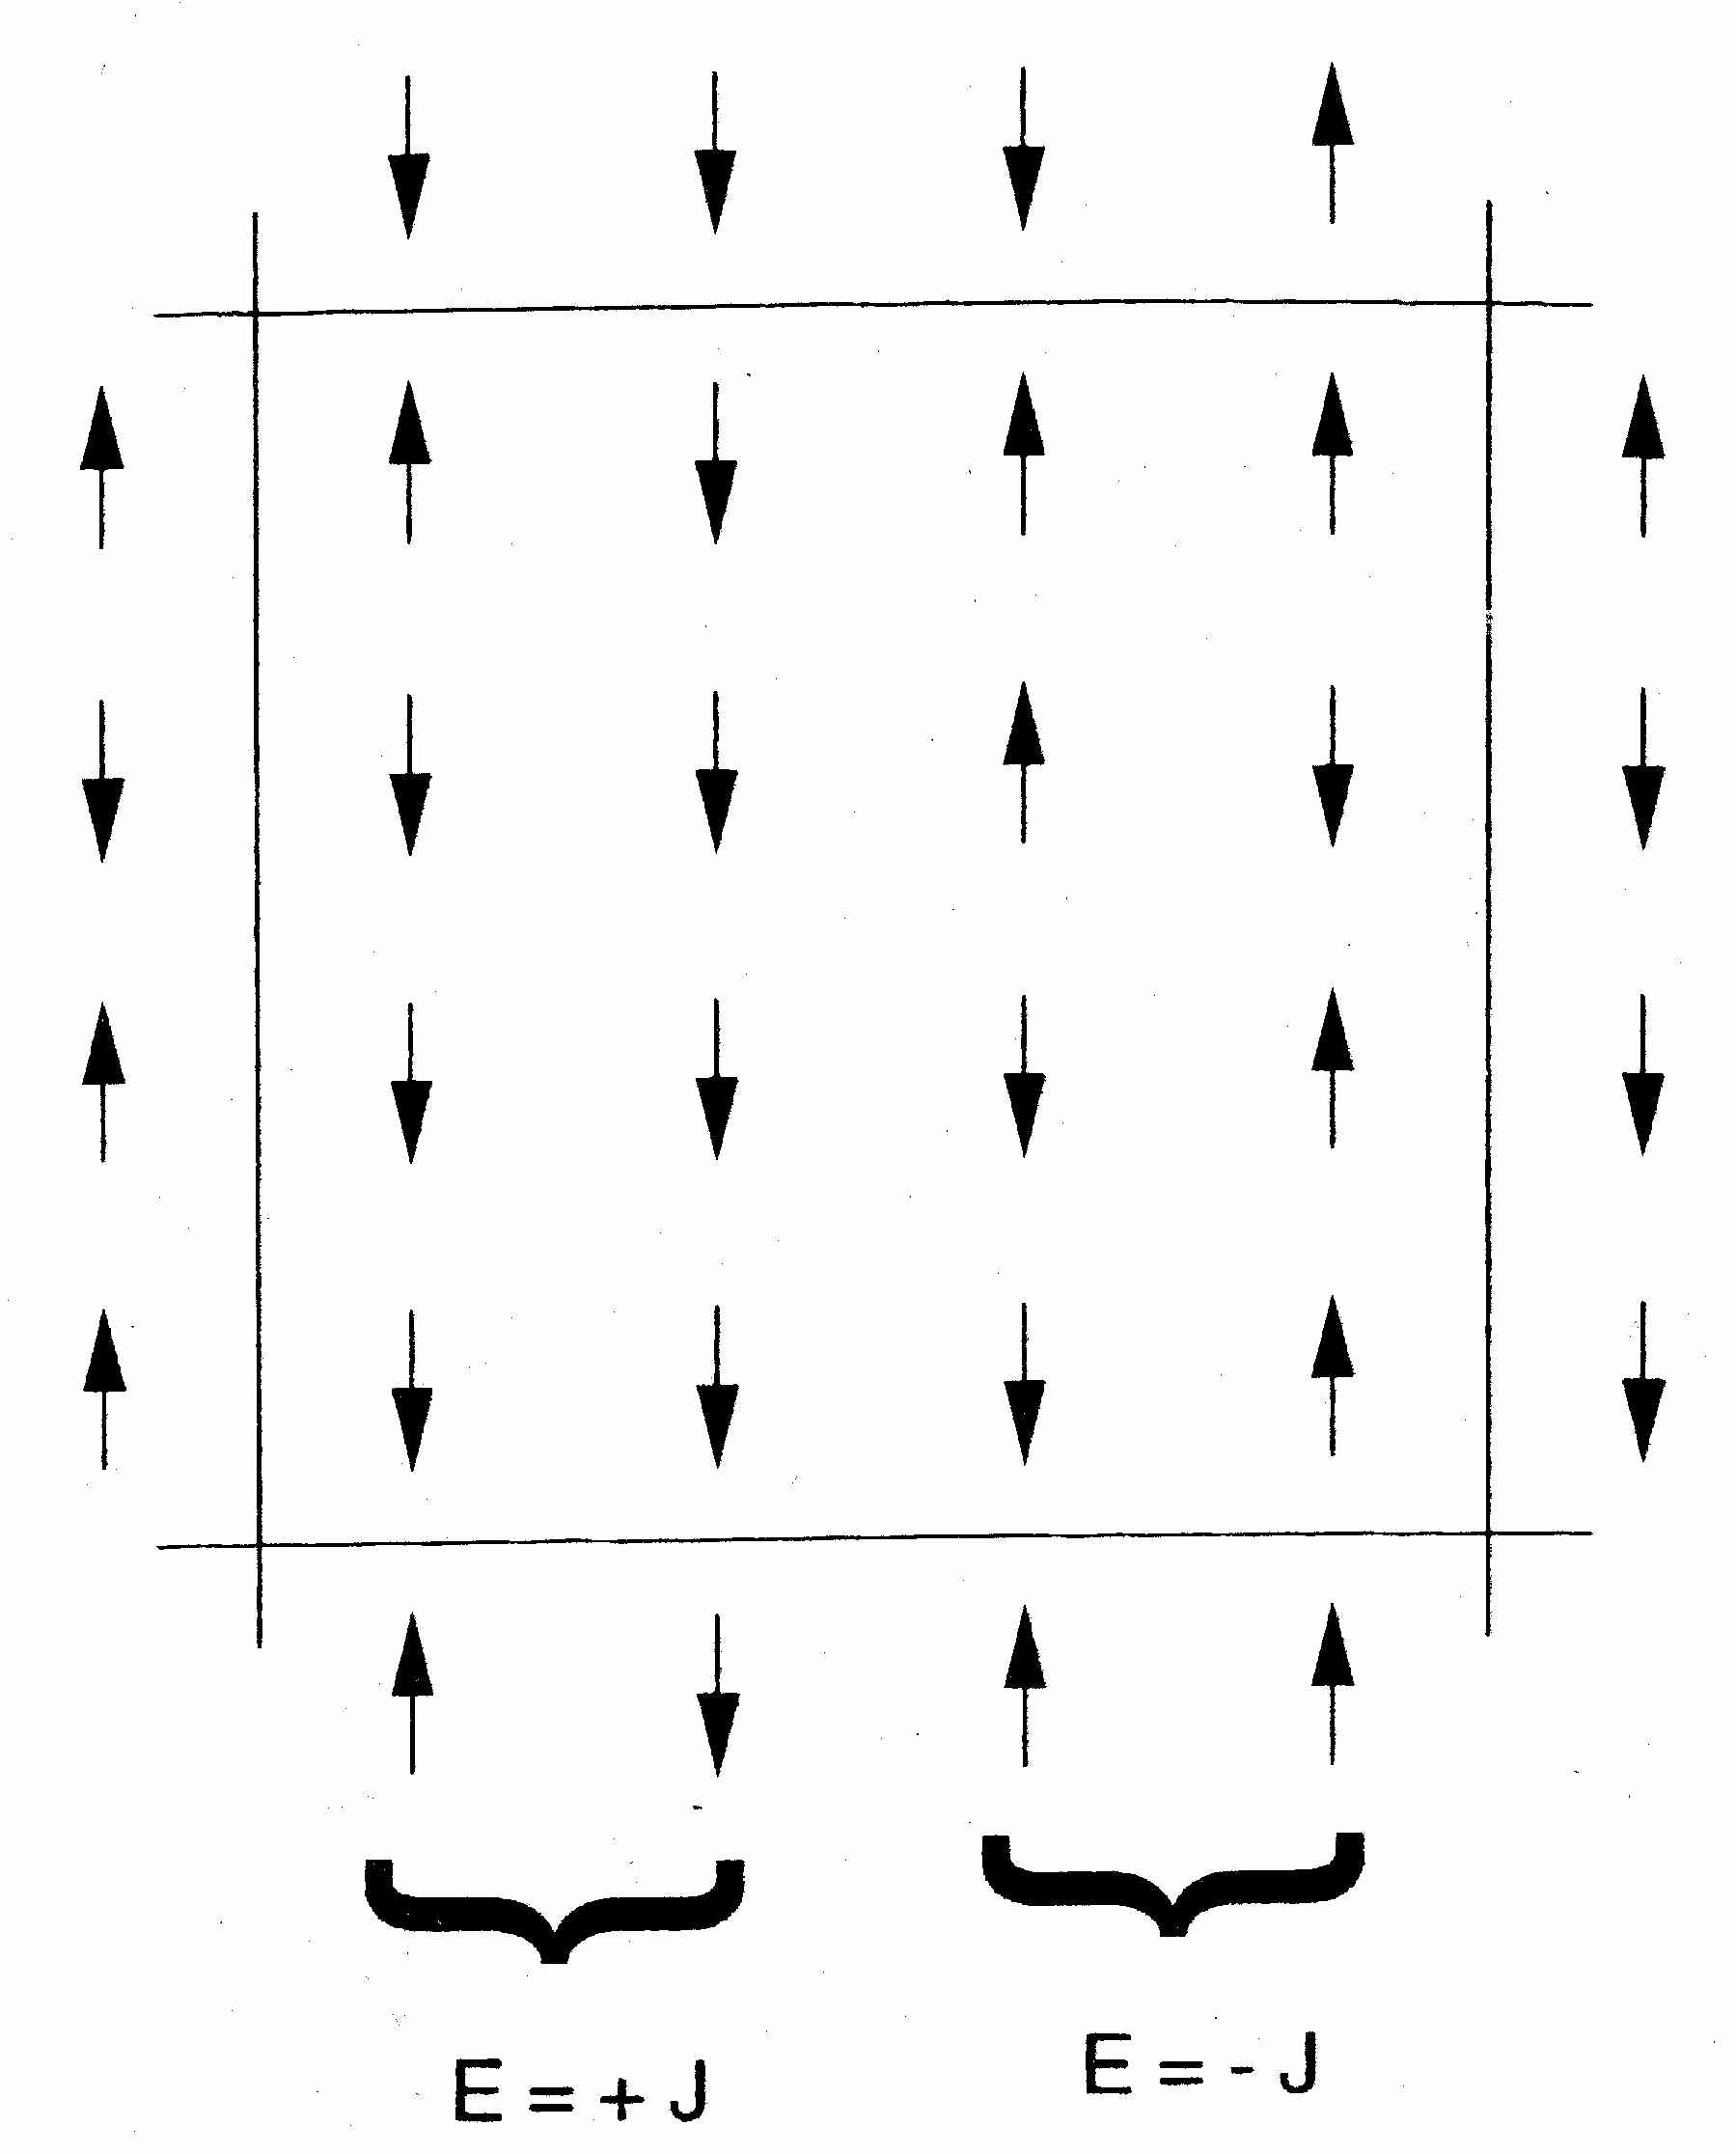
\includegraphics[width=0.8\linewidth]{lattice.jpg}

    \end{columns}

}


\frame
{
    \frametitle{Project 3: 2D Ising Model}

    \textbf{Project description:}

    \bigskip

    \begin{itemize}

        \item Simulate the 2D Ising spin lattice.

        \bigskip

        \item Implement the Monte Carlo Metropolis-Hastings algorithm.

        \bigskip

        \item Calculate properties such as heat capacity, magnetization, and magnetic susceptibility.

    \end{itemize}

}

\frame
{
    \frametitle{Project 4: Chemical Shifts Study}

    \begin{center}
        Using chemical shifts to determine protein structures.
    \end{center}

    \bigskip

%    \begin{columns}[c]
%
%        \column{0.5\textwidth}

            \centering
        
            \includegraphics[width=0.6\linewidth]{protein}\\
            \includegraphics[width=0.6\linewidth]{chemical_shift}


%        \column{0.5\textwidth}
%
%            \centering
%
%            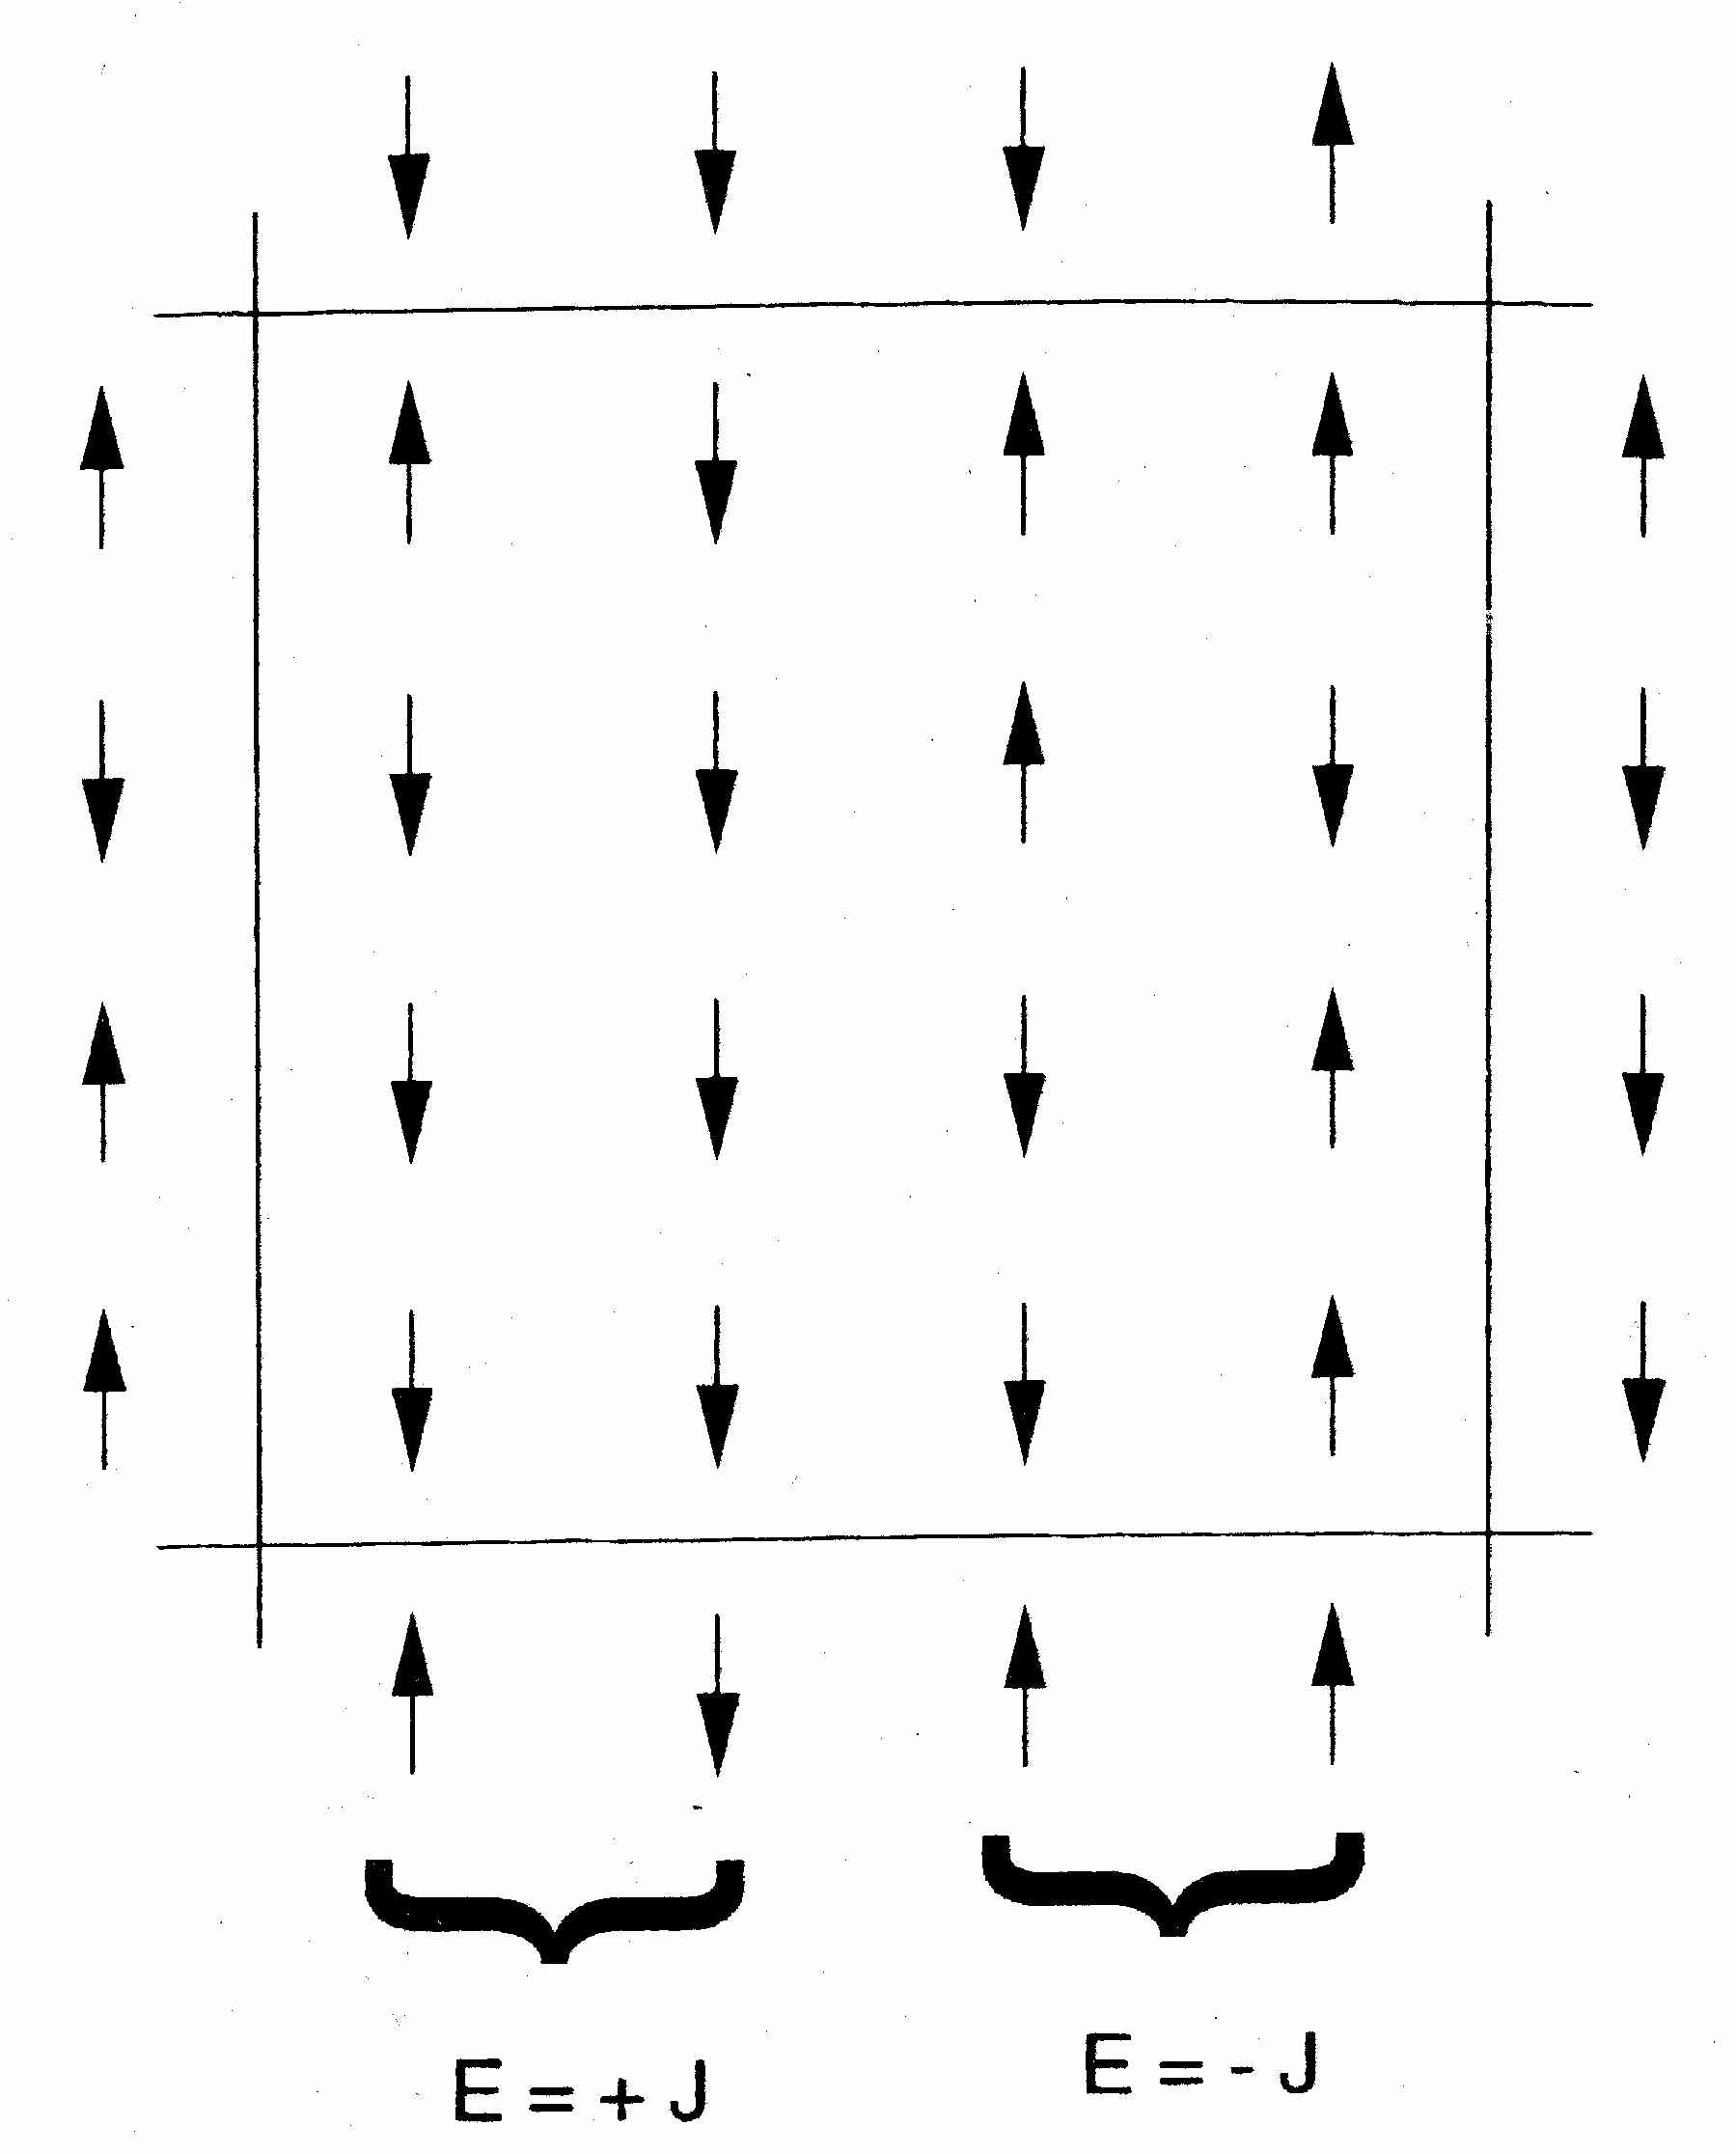
\includegraphics[width=0.8\linewidth]{lattice.jpg}

%    \end{columns}

}


\frame
{
    \frametitle{Project 3: 2D Ising Model}
    \frametitle{Project 4: Chemical Shifts Study}

    \textbf{Project description:}

    \bigskip

    \begin{itemize}

        \item Simulate the 2D Ising spin lattice.

        \bigskip

        \item Implement the Monte Carlo Metropolis-Hastings algorithm.

        \bigskip

        \item Calculate properties such as heat capacity, magnetization, and magnetic susceptibility.

    \end{itemize}

}

\frame
{

    \frametitle{Project description}

    \textbf{General:}

    \begin{itemize}

        \item Programming is done in small groups

        \item The reports are individual.

        \item The language is Danish or English.

    \end{itemize}

    \bigskip

    \textbf{Supervisor:}

    \begin{itemize}

        \item Jimmy is supervisor for {\bf Genetic Algorithm} and {\bf Diffusion}.

        \item Lars is supervisor for {\bf Ising-model}.

    \end{itemize}

    \bigskip

    \textbf{\code{if stuck}:}

    \begin{enumerate}

        \item Collaborate with other groups.

        \item Write an email and make an appointment to meet with\newline the supervisor.

    \end{enumerate}

}


% ***************************************************
% END FRAMES
% ***************************************************

\end{document}

